	\documentclass[]{standalone}
	\usepackage{tikz}
	\usetikzlibrary{math}
	
	\pgfkeys{
	 /testing/.is family,
	 /testing,
	  b/.store in =\b,  
	  a/.store in =\a}
	
	\newcommand{\testing}[1][]{\pgfkeys{/testing, #1}
	\tikzmath{
	real \a, \b;
	print ($Out:$);
	print ($a = \a,$);
	print ($b = \b |$);
	}}

	\begin{document}
	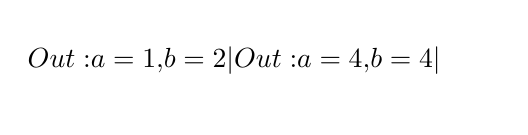
\begin{tikzpicture}
	\tikzmath{\b = 3;}
	\path(0,-0.5) -- (6,0.5);
	\testing[a = 1, b = 2]     %Result: a = 1, b = 2
	\testing[a = \b, b = 4]    %Result: a = 4, b = 4. I want it to be a = 3, b = 4.
	\end{tikzpicture}	
	\end{document}